%Describe all the related works
%Exhaustive Matching
%Chamfer Matching
%Will be intensive articles oriented.
%Harris Corner Detection
%Pattern based matching
%SIFT Corner Detectors
%SURF Corner Detectors
% OpenCV library
This chapter surveys previous work in image stitching. As already said in chapter~\ref{chapter:introduction}, algorithms for aligning images and stitching them into seamless photo-mosaics are the oldest and most widely used in computer vision. The first image stitching concept was known to be implemented to create panoramas in 1787 by \emph{Robert Barker}, an Irishman, who created panoramas of a cylindrical building~\cite{Woeste:09}.\\

\noindent In the past, exhaustive methods were used which calculate a measure of the difference between the images at all possible values in the search space. Those methods were time consuming. If we are registering two images: $I_1$ of size $M X M$ and $I_2$ of size $N X N$, then the computation complexity will be $O(M^2N^2)$ \footnote{matching for rotated images,complexity increases.}.Those methods were used for long time until \emph{Lucas and Kanade}'s patch-based translational alignment\cite{Lucas:81}. The registration method purposed by Lucas and Kanade~\cite{Lucas:81} became widely popular at that time because it drastically reduced the computational time to $O(M^2 log N)$. The matching process was an iterative \emph{Newton Raphson} method where we go on getting better match in each iteration. \\ 

\noindent Similarly, \emph{Xue Mei} and \emph{Fatih Porikli}~\cite{Mei:06} have purposed a computationally inexpensive method for multi-modal image registration. Their method employs a joint gradient similarity function that is applied only to a set of high spatial gradient pixels. They used the gradient ascent method to get the maximization of similarity function which gives the motion parameters for best match. \\ 

 

\noindent The edge based \emph{Chamfer matching} methods also became popular which used the edge information in the image for matching. In Chamfer matching, we select an image as template and try to match with other image using distance transform as shown in figure~\ref{fig:matching-dt}. We can use the various transformed templates to match rotated images~\cite{Gavrila:98}. Gavrilla and Philomin~\cite{Gavrila:99} implemented the Chamfer based matching method in real-time detection of traffic signs and pedestrians from a moving vehicle. They used coarse-to-fine approach over the shape hierarchy and over the transformation parameters to make the matching faster.\\ 

\begin{figure}%
\begin{center}
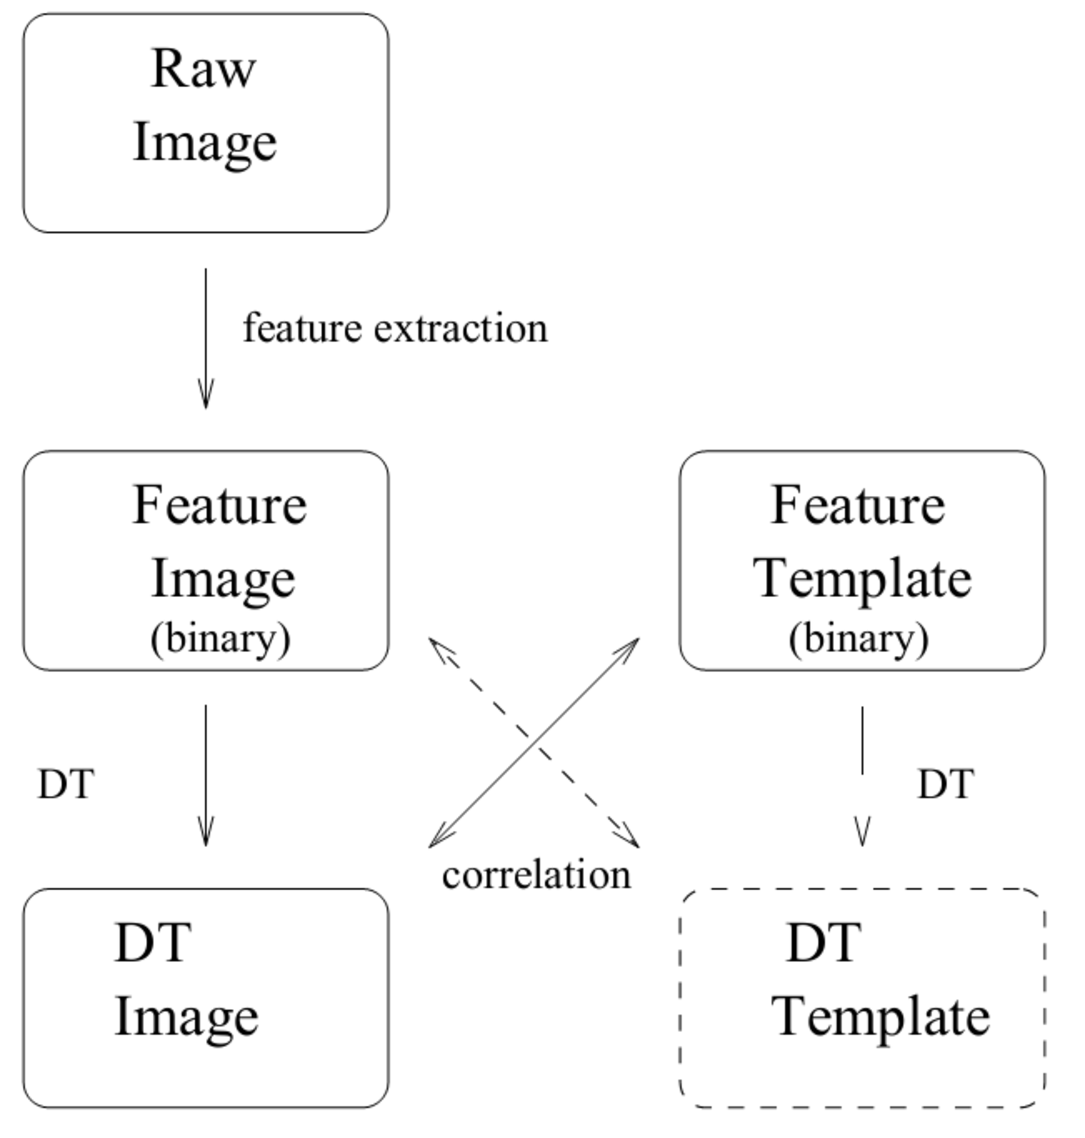
\includegraphics[width=0.5\columnwidth]{2.mainmatter/1.Introduction/figures/chamfer-matching}%
\caption[Matching Using a DT]{Matching using a distance transform. \imgsrc{(Image source: Gavrilla~\cite{Gavrila:98})}}%
\label{fig:matching-dt}%
\end{center}
\end{figure}

\noindent There are several research papers which describe the global image alignment methods. The computation of globally consistent alignments has been discussed in the literature by Szeliski and Shum~\cite{Szeliski:97} and the variations of exposure has been addressed by Sawhney \textit{et al}~\cite{Sawhney:99}.\\ 


\noindent More recent algorithms on image alignment extract a sparse set of feature points and match these points to each other to get the motion parameters~\cite{Szeliski:06}. \emph{Brown} and \emph{Lowe} in their paper~\cite{Brown:02} discusses on obtaining the invariant local features to find the matches between the images and they also claim the method to be insensitive to ordering, orientation, scale and illumination of input images. And there are several research papers which discuss on extracting the feature points in the image. Some basic corner detectors including \emph{Harris} have been discussed by Parks and Gravel~\cite{Parks:11}. Similarly, the very fast corner detector(\emph{Features from Accelerated Segment Test}) have been purposed by Rosten et al~\cite{Rosten:06}. The more robust feature points extractors (\emph{SIFT} and \emph{SURF}) has been discussed by Lowe~\cite{Lowe:04} and Bay et al~\cite{Bay:08}. The authors of the papers claim that those feature extractors are more robust and invariant to image rotation, scale or intensity changes. 





 